\newpage
\section{Programmablauf}
Im nachfolgendem Sequenzdiagramm wird dargestellt welche Methoden in welcher Klasse beim \"offnen einer Datei \"uber den Button in der Men\"uleiste ausgef\"uhrt werden:

\begin{figure}[h]
\centering
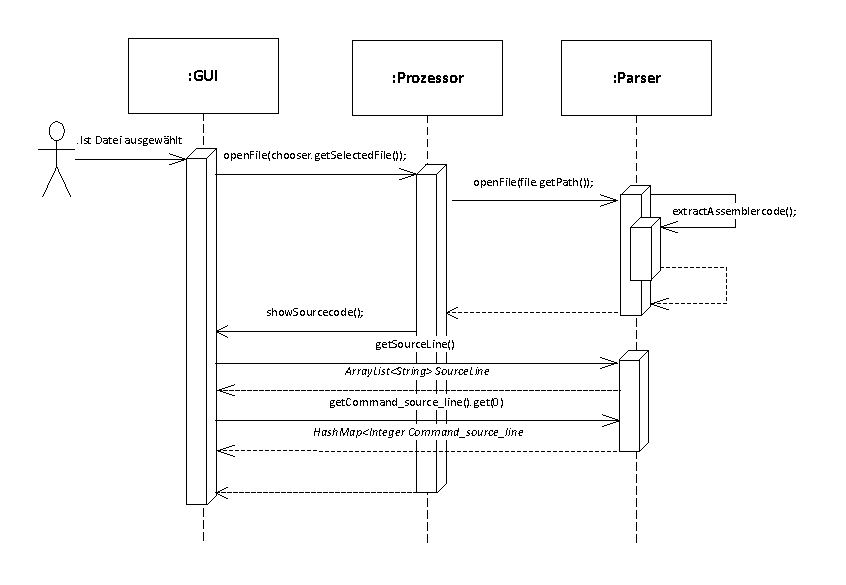
\includegraphics[scale=1]{Bilder/SeqOff.pdf}
\caption{Sequenzdiagramm f\"ur das \"Offnen und Parsen einer Datei}
\end{figure}

\noindent Die Methode showSourcecode(parser.getSourceLine(),
 parser. getCommand\\\_source\_line().get(0)) ruft als \"Ubergabeparameter die Methoden getSourceLine() und getCommand\_source\_ line() des Parsers auf. Diese \"Ubergabeparameter sind aus Platzgr\"unden nicht im Diagramm enthalten, werden aber trotzdem aufgerufen.
\\
\\\noindent Die Methode extractAssemblerCode() extrahiert aus der .lst Datei jeweils die Zeilen als String (SourceLine()) und den Befehlscode der ersten Zeichen (Command\_source\_ line()). In einer Schleife werden die String-Zeilen im User Interface ausgegeben.
\newpage

\lstinputlisting[language=java]{Listings/exA.java}

\noindent Durch das klicken des Go-Buttons beginnt die Simulation. Wie einzelne Befehle erkannt werden wird im folgendem Sequenzdiagramm dargestellt.

\begin{figure}[h]
\centering
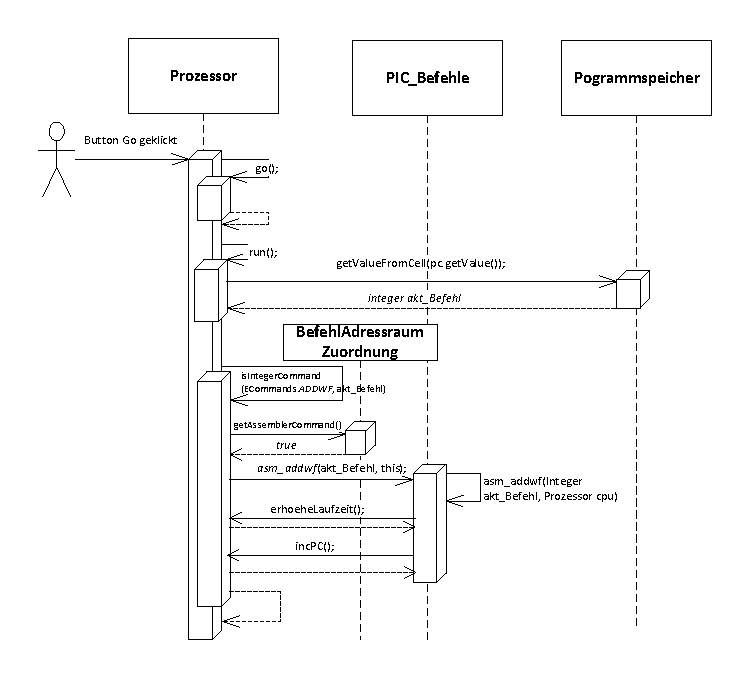
\includegraphics[scale=0.9]{Bilder/SeqBef.pdf}
\caption{Sequenzdiagramm f\"ur das Erkennen eines Befehls}
\end{figure}
\newpage
\noindent Durch den Go Befehl wir die Schrittweite des run Vorgangs ver\"andert und f\"angt nun an jeden Befehl zu erkennen und abzuarbeiten. Zun\"achst wird der aktuelle Befehl aus dem Programmspeicher geladen. Danach wird \"uberpr\"uft ob sich der aktuelle Befehl im Addressbereichsraum des Befehls ADDWF befindet.
In diese Beispiel liefert die Methode true zur\"uck und die eigentliche Ausf\"uhrungsroutine in der Klasse PIC\_Befehle wird aufgerufen. Nach dem Ausf\"uhren der Methode wird noch die Laufzeit und der Programm Counter erh\"oht.
\\
\\\noindent W\"urde der aktuelle Befehl nicht im Adressraum von ADDWF liegen w\"are der R\"uckgabewert false und die Methode w\"urde den textuell n\"achsten Adressraum eines Befehls \"uberpr\"ufen. Bei der Untersuchung jedes Befehls wird zus\"atzlich noch \"uber die Methode checkInterrupt(this) \"uberpr\"uft ob ein Interrupt stattgefunden hat.
 Wie die Abarbeitung der Befehle im genauen stattfindet wird im n\"achsten Kapitel n\"aher erl\"autert.
